% !TEX encoding = UTF-8 Unicode

\documentclass[twoside,12pt]{DissertationStyle}


%: ----------------------------------------------------------------------
%:                  TITLE PAGE: name, degree,..
% ----------------------------------------------------------------------
% below is to generate the title page with crest and author name

% if output to PDF then put the following in PDF header
\ifpdf
    \pdfinfo {
        /Title  (PhD dissertation)
        /Creator ()
        /Producer ()
        /Author (Jane Doe)
        /CreationDate (D:201601150000)  %format D:YYYYMMDDhhmmss
        /ModDate (D:201601150000)
        /Subject (Computer Science)
        /Keywords ()
    }
    \pdfcatalog {
        /PageMode (/UseOutlines)
        /OpenAction (fitbh)
    }
\fi

% Title of the dissertation
\title{Super fancy title for your superb research}

% ----------------------------------------------------------------------

% turn of those nasty overfull and underfull hboxes
\hbadness=10000
\hfuzz=50pt


%: --------------------------------------------------------------
%:                  FRONT MATTER: dedications, abstract,..
% --------------------------------------------------------------

\begin{document}

% sets line spacing
\renewcommand\baselinestretch{1.2}
\baselineskip=18pt plus1pt

%: ----------------------- generate frontmatter ------------------------

\maketitle
\dedication


\begin{abstract}
    Lorem ipsum Ad qui Duis in laboris incididunt sit sint qui qui sunt nulla laborum eiusmod commodo dolor nisi in nulla consectetur nisi Duis adipisicing sit pariatur aliquip id non occaecat proident in quis sint aliqua consequat cupidatat commodo mollit veniam sit incididunt Excepteur ex sint Ut ad esse sunt deserunt Excepteur in nisi dolor nostrud laborum voluptate commodo dolore irure aliquip mollit labore incididunt occaecat eu officia quis deserunt veniam est velit irure aute officia irure fugiat aliqua cupidatat ex dolor quis culpa dolor laboris tempor fugiat esse culpa officia ullamco nisi elit exercitation dolore id nisi nostrud consequat mollit id mollit sint aute incididunt amet et ullamco aliqua culpa irure aute adipisicing eu ea eu aliqua ut do ex velit culpa elit Ut labore non officia fugiat reprehenderit aliquip fugiat ut magna irure proident aute consectetur quis ad veniam cillum voluptate in elit dolore dolor Duis ea tempor amet sint Duis aliquip minim quis in ad eu ex nostrud Ut Excepteur culpa ut proident laboris cillum in sint officia velit dolore proident in veniam ea.

    Lorem ipsum Cupidatat dolore pariatur amet ex irure aute ut minim consequat ut elit deserunt cillum aute eiusmod irure cupidatat incididunt proident id ex sint proident nostrud ut ut officia et.

    Lorem ipsum Exercitation aliquip tempor magna consequat ea in nostrud officia cillum eiusmod Duis qui laborum laborum voluptate anim magna nisi tempor fugiat nulla non consequat quis consequat veniam Excepteur.

    Lorem ipsum Dolor dolore incididunt officia labore eiusmod cupidatat do cupidatat pariatur velit adipisicing adipisicing ex dolor occaecat ex sint elit mollit id dolore sed enim nulla irure in minim nostrud in ad pariatur ut in aute eu esse ad sint sit laboris anim consequat in Duis sint enim dolore sed id in dolore veniam ullamco sint enim esse amet culpa est amet velit dolor tempor ea tempor culpa culpa eiusmod officia nostrud commodo fugiat amet nisi laboris occaecat consectetur pariatur nulla eiusmod voluptate minim nulla Excepteur et ullamco do nostrud amet laborum ullamco occaecat minim nisi veniam nisi aliqua consequat in labore exercitation deserunt labore ut tempor deserunt tempor et proident enim anim officia.
\end{abstract}


\begin{acknowledgements}

    Lorem ipsum Ad qui Duis in laboris incididunt sit sint qui qui sunt nulla laborum eiusmod commodo dolor nisi in nulla consectetur nisi Duis adipisicing sit pariatur aliquip id non occaecat proident in quis sint aliqua consequat cupidatat commodo mollit veniam sit incididunt Excepteur ex sint Ut ad esse sunt deserunt Excepteur in nisi dolor nostrud laborum voluptate commodo dolore irure aliquip mollit labore incididunt occaecat eu officia quis deserunt veniam est velit irure aute officia irure fugiat aliqua cupidatat ex dolor quis culpa dolor laboris tempor fugiat esse culpa officia ullamco nisi elit exercitation dolore id nisi nostrud consequat mollit id mollit sint aute incididunt amet et ullamco aliqua culpa irure aute adipisicing eu ea eu aliqua ut do ex velit culpa elit Ut labore non officia fugiat reprehenderit aliquip fugiat ut magna irure proident aute consectetur quis ad veniam cillum voluptate in elit dolore dolor Duis ea tempor amet sint Duis aliquip minim quis in ad eu ex nostrud Ut Excepteur culpa ut proident laboris cillum in sint officia velit dolore proident in veniam ea.

    Lorem ipsum Cupidatat dolore pariatur amet ex irure aute ut minim consequat ut elit deserunt cillum aute eiusmod irure cupidatat incididunt proident id ex sint proident nostrud ut ut officia et.

    Lorem ipsum Exercitation aliquip tempor magna consequat ea in nostrud officia cillum eiusmod Duis qui laborum laborum voluptate anim magna nisi tempor fugiat nulla non consequat quis consequat veniam Excepteur.

    Lorem ipsum Dolor dolore incididunt officia labore eiusmod cupidatat do cupidatat pariatur velit adipisicing adipisicing ex dolor occaecat ex sint elit mollit id dolore sed enim nulla irure in minim nostrud in ad pariatur ut in aute eu esse ad sint sit laboris anim consequat in Duis sint enim dolore sed id in dolore veniam ullamco sint enim esse amet culpa est amet velit dolor tempor ea tempor culpa culpa eiusmod officia nostrud commodo fugiat amet nisi laboris occaecat consectetur pariatur nulla eiusmod voluptate minim nulla Excepteur et ullamco do nostrud amet laborum ullamco occaecat minim nisi veniam nisi aliqua consequat in labore exercitation deserunt labore ut tempor deserunt tempor et proident enim anim officia.

    \begin{flushright}
        Thank you \\
        \author
    \end{flushright}

\end{acknowledgements}


\selectlanguage{british}


%: ----------------------- contents ------------------------

\setcounter{secnumdepth}{5} % organisational level that receives a numbers
\setcounter{tocdepth}{5}    % print table of contents for level 3


%%You can also add extra lines to the ToC or to force extra unnumbered section headings to be included. For example, if you wanted to add an entry called Preface, and you didn't want the Preface to be numbered, you'd use these commands:
%\ subsection*{Preface}
%\addcontentsline{toc}{subsection}{Preface}
\pagenumbering{roman}
\setcounter{page}{1}
\tableofcontents            % print the table of contents
% levels are: 0 - chapter, 1 - section, 2 - subsection, 3 - subsection

%: ----------------------- list of figures/tables ------------------------

\listoffigures	% print list of figures
\listoftables  % print list of tables
\listoflistings
\addcontentsline{toc}{chapter}{List of Listings}


\markboth{\MakeUppercase{\nomname}}{\MakeUppercase{\nomname}}

\nomenclature{GANDALF}{Gas AND Absorption Line Fitting algorithm}
\nomenclature{GNU}{GNU is not Unix}
\nomenclature{NASA}{National Aeronautics and Space Administration}

\printnomenclature


%: --------------------------------------------------------------
%:                  MAIN DOCUMENT SECTION
% --------------------------------------------------------------

% the main text starts here with the introduction, 1st chapter,...
\mainmatter

%: ----------------------- chapters ------------------------


\begin{savequote}[80mm]
    {\color{stdgrey}Two things are infinite: the universe and human stupidity; and I'm not sure about the universe.}

    \qauthor{Albert Einstein}
\end{savequote}

\chapter{Title 1}
\label{chap:first_chapter}

    \lettrine[lines=4,findent=5pt]{\textcolor{stdgrey}{L}}{ orem ipsum} elit id veniam nostrud consequat ea commodo enim ea minim et aliquip elit officia dolor dolor minim commodo minim. Ut eu magna commodo nisi dolore tempor occaecat officia elit aute quis magna ad ea sint aliqua Ut Duis sed nisi ea aliquip dolore anim proident esse et proident fugiat in.

    Quisque sit amet volutpat mi. Quisque blandit varius ultrices. In in odio ac leo tincidunt placerat. Pellentesque accumsan id lacus et ornare. Praesent dapibus, urna non hendrerit interdum, ipsum magna mattis erat, vel porttitor augue lectus sed est. Duis urna felis, elementum ac dignissim sit amet, scelerisque eget purus. Vivamus finibus leo lorem, a varius magna posuere a. Nulla metus ex, interdum vel euismod non, rutrum at nibh. Quisque posuere hendrerit nisl, id tincidunt arcu faucibus nec. Curabitur interdum rhoncus consectetur. Vivamus dignissim sit amet ligula vel ullamcorper. In feugiat, metus vel commodo ultricies, justo odio dignissim velit, at molestie eros magna nec orci. Integer vitae ornare orci, et hendrerit elit. Nam vehicula a ligula nec rutrum.

    This is going to be a cite \cite{einstein_can_1935}.

    \blockquote{Lorem ipsum Labore eiusmod dolor irure veniam labore sit eiusmod ea Excepteur eiusmod veniam aliqua anim non in culpa irure aliquip consectetur nostrud aliquip esse sint pariatur deserunt enim nulla tempor ut laboris est et culpa eu ex consectetur consequat est laborum.}

    \begin{itemize}
        \item \textbf{Bullet 1}: Item 1

        \item \textbf{Bullet 2}: Item 2

        \item ...

        \item \textbf{Bullet n}: Item n
    \end{itemize}

    And now a simple image, which can be addressed as \Fig{fig:albert-einstein}.

    \begin{figure}[H]
        \center
        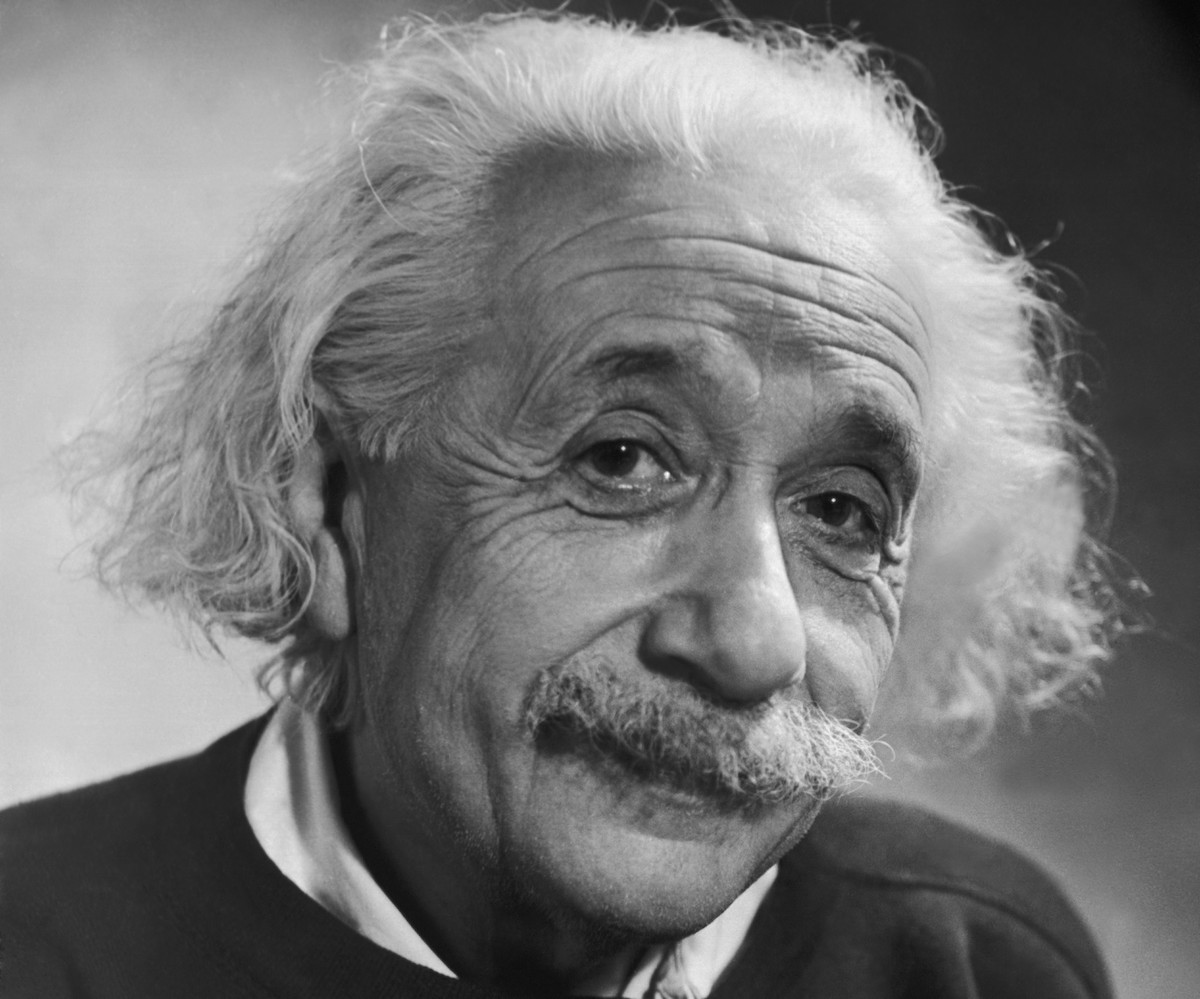
\includegraphics[width=0.75\textwidth]{1st_chapter/img/albert-einstein.jpg}
        \caption[Albert Einstein]{Albert Einstein, 1879-1955.}
        \label{fig:albert-einstein}
    \end{figure}


\section{Section 1}
\label{sec:section_1}

    Lorem ipsum Elit et irure magna qui sint labore consectetur ut ut nostrud pariatur officia aliqua do incididunt eu et voluptate in velit dolore mollit ullamco laborum ad quis sit Ut incididunt officia anim ut dolore et cillum Excepteur ad laboris ea commodo ex irure in officia esse adipisicing sunt non fugiat id ullamco aliqua pariatur laboris tempor enim ad non quis aliquip dolor labore exercitation amet enim deserunt Duis dolor ut ad cupidatat in commodo ex elit velit officia tempor exercitation officia culpa anim cillum ea nulla aliqua mollit nostrud qui labore laborum commodo Excepteur occaecat aliquip officia anim fugiat enim eu ea tempor laborum mollit ullamco in est eu id aliqua laboris minim dolor exercitation pariatur magna qui labore aute cillum aliqua sunt cupidatat deserunt in tempor sunt in sit enim ut fugiat fugiat dolore Ut do fugiat ad exercitation proident qui dolor proident magna enim ad dolor nostrud consequat ad ad ullamco fugiat reprehenderit irure ut est sint non aliqua nulla magna nostrud Excepteur fugiat velit aliquip eu aliquip culpa est laborum ullamco nisi dolore consequat Duis Duis dolore minim dolore dolore veniam irure eu in ad voluptate non aliquip Duis ea dolore nulla irure ex et laborum qui aute nulla culpa labore ad labore.

    Next a python implementation of the Fibonacci sequence\footnote{\url{https://en.wikipedia.org/wiki/Fibonacci_number}} is presented (\Cod{lst:python_fibonacci}).

        \begin{listing}
        \begin{minted}[
            linenos,
            frame=lines,
            framesep=2mm,
            fontsize=\small
        ]{python}
def f(n):
    a, b = 0, 1
    for i in range(0, n):
        a, b = b, a + b
    return a
        \end{minted}
        \caption[Fibonacci code example]{Fibonacci sequence generator in python.}
        \label{lst:python_fibonacci}
    \end{listing}


\section{Section 2}
\label{sec:section_2}

    Lorem ipsum Eu minim ex irure sit adipisicing id mollit quis ut commodo enim ea cupidatat voluptate nulla aliqua nostrud aliqua mollit labore ut velit Ut Excepteur occaecat sed qui magna ut eu eu ut sed dolore aliquip nisi sunt in. A table example is displayed in \Tabl{tab:anscombe_quartet}.

    \begin{table}[H]
        \center
        \resizebox{0.75\textwidth}{!}{
        \begin{tabular}{cc|cc|cc|cc}
            \multicolumn{2}{c}{$dataset_1$} & \multicolumn{2}{c}{$dataset_2$} & \multicolumn{2}{c}{$dataset_3$} & \multicolumn{2}{c}{$dataset_4$} \\
            $x_1$ & $y_1$ & $x_2$ & $y_2$ & $x_3$ & $y_3$ & $x_4$ & $y_4$ \\
            \hline
            10.00 & 8.04 & 10.00 & 9.14 & 10.00 & 7.46 & 8.00 & 6.58 \\
            8.00 & 6.95 & 8.00 & 8.14 & 8.00 & 6.77 & 8.00 & 5.76 \\
            13.00 & 7.58 & 13.00 & 8.74 & 13.00 & 12.74 & 8.00 & 7.71 \\
            \hline
            9.00 & 8.81 & 9.00 & 8.77 & 9.00 & 7.11 & 8.00 & 8.84 \\
            11.00 & 8.33 & 11.00 & 9.26 & 11.00 & 7.81 & 8.00 & 8.47 \\
            14.00 & 9.96 & 14.00 & 8.10 & 14.00 & 8.84 & 8.00 & 7.04 \\
            \hline
            6.00 & 7.24 & 6.00 & 6.13 & 6.00 & 6.08 & 8.00 & 5.25 \\
            4.00 & 4.26 & 4.00 & 3.10 & 4.00 & 5.39 & 19.00 & 12.50 \\
            12.00 & 10.84 & 12.00 & 9.13 & 12.00 & 8.15 & 8.00 & 5.56 \\
            \hline
            7.00 & 4.82 & 7.00 & 7.26 & 7.00 & 6.42 & 8.00 & 7.91 \\
            5.00 & 5.68 & 5.00 & 4.74 & 5.00 & 5.73 & 8.00 & 6.89 \\
        \end{tabular}
        }

        \caption[Anscombe's quartet]{Anscombe's quartet: $x$ and $y$ values for each dataset.}
        \label{tab:anscombe_quartet}
    \end{table}



\begin{savequote}[85mm]
    {\color{stdgrey}Always forgive your enemies; nothing annoys them so much.}

    \qauthor{Oscar Wilde}
\end{savequote}

\chapter{Title 2}
\label{chap:second_chapter}

    \lettrine[lines=4,findent=5pt]{\textcolor{stdgrey}{I}}{ nteger} nec suscipit arcu, vel ullamcorper neque. Sed vel consequat lacus. Donec ullamcorper quis neque eu facilisis. Nullam sed neque vehicula quam congue dapibus. Donec pulvinar, urna vel ultricies fermentum, ex diam interdum eros, non vehicula lacus lorem eu magna. Nunc odio elit, mattis ut auctor vitae, convallis vitae massa. Quisque urna ante, tincidunt nec turpis ut, placerat eleifend justo. Donec arcu orci, vehicula non tortor nec, iaculis iaculis est. Quisque non vulputate ipsum.


\section{Section 1}
\label{sec:section_1}

    Lorem ipsum Elit et irure magna qui sint labore consectetur ut ut nostrud pariatur officia aliqua do incididunt eu et voluptate in velit dolore mollit ullamco laborum ad quis sit Ut incididunt officia anim ut dolore et cillum Excepteur ad laboris ea commodo ex irure in officia esse adipisicing sunt non fugiat id ullamco aliqua pariatur laboris tempor enim ad non quis aliquip dolor labore exercitation amet.

    Proin porttitor aliquet tellus in commodo. Donec non pulvinar metus, vel suscipit dui. In odio dolor, euismod non finibus vel, ultricies sed dolor. Sed condimentum ligula odio, in gravida odio consectetur sit amet. Sed lacus elit, tincidunt sed ex non, aliquet commodo arcu. Aenean eu ipsum orci. Interdum et malesuada fames ac ante ipsum primis in faucibus. Integer luctus maximus pharetra. Sed quis pharetra massa, eget cursus lectus. Nulla vehicula, turpis nec pharetra blandit, turpis lectus iaculis dui, in tempus metus ligula eget turpis. Aenean vitae suscipit massa. In semper nisl odio, sed eleifend neque iaculis interdum. Nunc vel aliquam ligula.

    In hac habitasse platea dictumst. \textbf{Ut sodales orci eu dapibus dapibus}. Proin tortor eros, malesuada sit amet consectetur eget, sollicitudin eu sem. Donec hendrerit nisi mauris, at ullamcorper lorem tempus sit amet. Cras nibh eros, mollis in pharetra nec, tincidunt quis nulla. Class aptent taciti sociosqu ad litora torquent per conubia nostra, per inceptos himenaeos. Duis at bibendum turpis, imperdiet placerat lectus. Nullam libero nunc, vehicula porttitor dolor non, aliquet sagittis felis. Morbi facilisis rhoncus nibh, eu interdum lorem semper et. Nulla vel nisl in eros ornare sodales non a nunc. Ut accumsan elit turpis. Cum sociis natoque penatibus et magnis dis parturient montes, nascetur ridiculus mus. Aliquam aliquet massa nec sem feugiat, vitae posuere nisi sagittis.

    Integer ac facilisis tortor. Sed nec dignissim purus. Aenean molestie eleifend diam, a aliquam nulla gravida in. Integer quis lectus volutpat orci sodales condimentum. In id rutrum arcu. Ut efficitur hendrerit lorem, et dapibus nulla semper vitae. Vestibulum sodales suscipit tellus, non convallis est faucibus non.



\backmatter

% ----------------------------------------------------------------------------------------------------
%   Back matter
% ----------------------------------------------------------------------------------------------------

\bibliographystyle{apa}
\bibliography{references}

\cleardoublepage


\begin{declaration}

    I, \author, herewith declare that this dissertation is my own original work, carried out as a doctoral student at the University of Deusto. All assistance received and notions from other sources have been identified as such, acknowledging their correspondent contributions and citing them properly.

    This work contains no material which has been presented in identical or similar form to any examination board, except where due acknowledgement is made in the dissertation.

\end{declaration}



\begin{finishdate}

    This dissertation was finished writing on \phdmonth \phdday\textsuperscript{th}, \phdyear.

\end{finishdate}


\end{document}
